%
% Modified by Megan Patnott
% Last Change: Jan 18, 2013
%
%%%%%%%%%%%%%%%%%%%%%%%%%%%%%%%%%%%%%%%%%%%%%%%%%%%%%%%%%%%%%%%%%%%%%%%%
%
% Modified by Sameer Vijay
% Last Change: Tue Jul 26 2005 13:00 CEST
%
%%%%%%%%%%%%%%%%%%%%%%%%%%%%%%%%%%%%%%%%%%%%%%%%%%%%%%%%%%%%%%%%%%%%%%%%
%
% Sample Notre Dame Thesis/Dissertation
% Using Donald Peterson's ndthesis classfile
%
% Written by Jeff Squyres and Don Peterson
%
% Provided by the Information Technology Committee of
%   the Graduate Student Union
%   http://www.gsu.nd.edu/
%
% Nothing in this document is serious except the format.  :-)
%
% If you have any suggestions, comments, questions, please send e-mail
% to: ndthesis@gsu.nd.edu
%
%%%%%%%%%%%%%%%%%%%%%%%%%%%%%%%%%%%%%%%%%%%%%%%%%%%%%%%%%%%%%%%%%%%%%%%%


%
% Chapter 2
%

\chapter{EXPERIMENTAL APPROACH}

\section{Experimental Objective}

\section{Experimental Facility}
Baseline acoustic measurements without plasma flow control were obtained in the Notre Dame Anechoic Wind Tunnel Facility (ND AWT). The ND AWT is a low-noise, open-jet acoustic wind tunnel with a free jet test section measuring 24-in-(0.610 m)-high by 24-in-(0.610 m)-wide installed in a large anechoic chamber suitable for frequencies above 100 Hz. The maximum empty test section velocity is approximately $U_\infty = 35$ m/s. The maximum safe tunnel velocity with the Notre Dame G550 Nose Landing Gear 30\%-scale model (ND G550) installed is  30 m/s corresponding to a Mach number of $M_\infty=0.1$.

Atmospheric properties such as ambient temperature and pressure were acquired using a digital thermometer and barometer. The tunnel speed is measured using a pitot-static probe installed approximately 6 in (0.154 m) from the free jet inlet centerline. From these data local sonic speed and the flow Mach number is computed.

\begin{figure}
\begin{center}
\begin{subfigure}{0.45\textwidth}
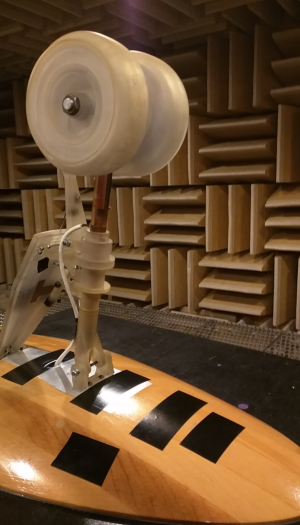
\includegraphics[width=\linewidth]{figures/model1a}
\caption{Baseline 1}
\label{fig:mod1a}
\end{subfigure}
\hspace*{\fill} % separation between the subfigures
\begin{subfigure}{0.45\textwidth}
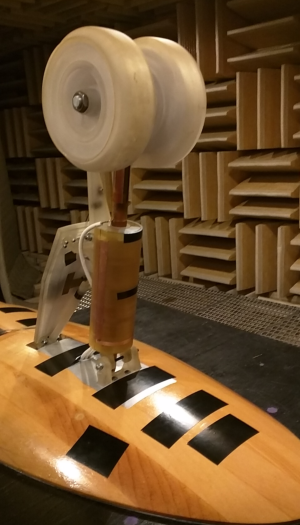
\includegraphics[width=\linewidth]{figures/model1b}
\caption{Baseline 2}
\label{fig:mod1b}
\end{subfigure}
\caption{ND G550 model with and without plasma fairing installed.}
\end{center}
\end{figure}

\section{Notre Dame G550 Nose Landing Gear Model}
Acoustic measurement for two baseline landing gear model configurations were performed. The first, designated Baseline 1, consisted of the ND G550 model without the plasma fairing installed, which is shown in the photograph of Figure \ref{fig:mod1a}. The second, designated Baseline 2, involved the ND G550 model retrofitted with a plasma fairing assembly in order to facilitate installation of dielectric barrier discharge (DBD) plasma actuators for flow control. This configuration is shown in the photograph of Figure \ref{fig:mod1b}. None of the acoustic measurements presented in this report for both configurations involved the use of plasma flow control. Rather, the focus was on the characterization of baseline acoustics for both configurations.

\section{Flow Visualization}

\section{Pressure Measurements}

\section{Microphone Measurements}
A polar array of omnidirectional microphones was used to acquire far field noise level spectra along the length of the AWT test section. It consists of a 1/2-in ACO Model 7046 electret microphone with companion 4012 preamplifier and PS9200 power supply. A schematic illustrating the array is shown in Figure \ref{fig:array}. Additionally, the array configuration relative to the G550 model is shown in the photograph of Figure \ref{fig:arraypic}. The microphone is mounted using a microphone stand so as to protrude from an acoustically treated rail by approximately 13 in (0.330 m). The total range of acoustic source-to-microphone angle spanned by the polar array is approximately $30^\circ \leq \theta \leq 150^\circ$ as referenced from the upper torque arm of the model in the downstream flow direction. As shown in Figure \ref{fig:arraypic}, the polar array is situated along the length of the free jet test section and positioned at the same height as the upper torque arm of the model, with the plane of the microphone located approximately 59 in (1.50 m) from the test section centerline.

\begin{figure}
	\begin{center}
		\centerline{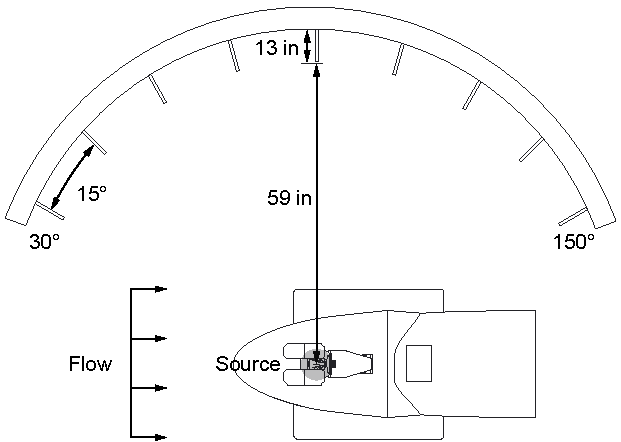
\includegraphics[scale=1.0]{figures/array_schematic}}
		\caption{Schematic of the polar array.}
		\label{fig:array}
	\end{center}
\end{figure}

\begin{figure}
	\begin{center}
		\centerline{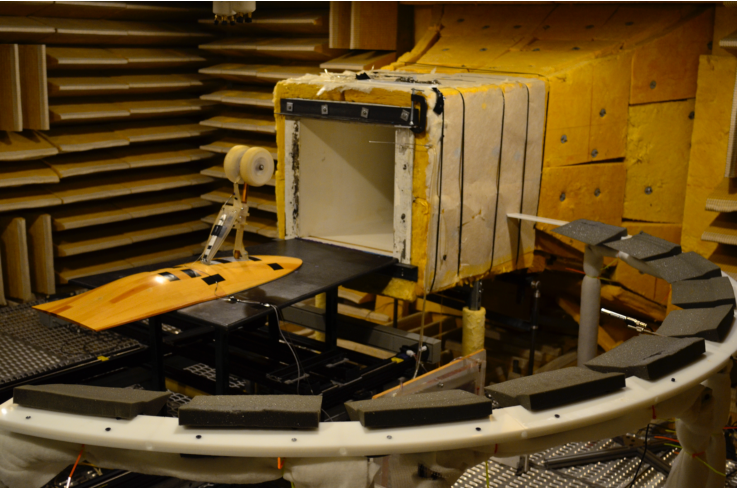
\includegraphics[scale=1.0]{figures/arraypic}}
		\caption{Photograph of the polar array installed in the ND AWT.}
		\label{fig:arraypic}
	\end{center}
\end{figure}


\section{Data Acquisition}
For microphone data acquisition, a National Instruments USB-6343 DAQ was used, yielding a total of 45 available channels with 48-bit ADC. The sampling parameters for the microphone data acquisition are listed in Table \ref{tab:data}.

\begin{table}
 \setlength{\capwidth}{0.8\textwidth}
\begin{center}
\caption{Data acquisition parameters.}
\label{tab:data}
\begin{tabular}{cccccccc}\toprule
\parbox{0.1\linewidth}{\centering Sensors} & 
\parbox{0.12\linewidth}{\centering Sampling Rate (Hz)} & 
\parbox{0.1\linewidth}{\centering $\frac{Samples} {block}$} & 
\parbox{0.11\linewidth}{\centering Window Function} & 
\parbox{0.1\linewidth}{\centering Overlap (\%)} & 
\parbox{0.1\linewidth}{\centering $N_{blocks}$} & 
\parbox{0.1\linewidth}{\centering $N_{averages}$} & 
\parbox{0.11\linewidth}{\centering Acquisition Time (s)} \\ \midrule
ACO & 65,536 & 2048 & Hanning & 0 & 960 & 960 & 30 \\ \bottomrule
\end{tabular}
\end{center}
\end{table}

\section{Current Results}

%In preparation for reading this dissertation, I would highly recommend
%reading some of the other material available on
%Gnus~\citep{gnus98:_gerry_ganst,greenfield96:_gettin_know_gnu}.  They
%are very well written and will give you a fuller understanding of
%Gnus.
%
%Gnus are frequently mistakes for squirrels.  They are not squirrels.
%They are Gnus.  Don't call them squirrels, either (unless you have
%food in your hand); they tend to get a bit upset.\footnote{This is
%  frequently mistaken for the chattering and scampering away.  Gnus
%  are actually quite polite; they will leave if they have nothing nice
%  to say, for fear of saying something offensive.}  If you have food
%in your hand, they tend to ignore this insult and accept your food as
%a peace offering.\footnote{Sometimes they'll follow you if you continue
%to refuse to feed them.}

%Table~\ref{tbl:bogus1} shows some feeding frequencies for where Gnus
%like to eat around the Notre Dame campus.  Gnus have work weeks, just
%like humans do, hence the much lower frequencies on weekends.  This
%can lead us to conclude that Gnu weekend shifts are much smaller than
%the normal work-week shifts.  In fact, we can attempt to parametrize the
%sighting frequency, $\mathcal{F}$, by the student population, type of food, and
%day of the week as:
%\begin{equation}
%  \mathcal{F} = \mathcal{F}(p,f,d).
%\end{equation}
%Table~\ref{tbl:bogus2} shows what they
%typically like to eat.
%
%\begin{table}[tpb]
%  \begin{center}
%    \caption{WHERE Gnus LIKE TO EAT \label{tbl:bogus1}}
%    \begin{tabularx}{0.85\textwidth}{lrrrrrrr} \toprule
%      \multicolumn{1}{c}{Location} & Sun & Mon & Tue & Wed & Thu & Fri & Sat \\ \midrule
%      Front of Dome & 1 & 5 & 6 & 5 & 4 & 5 & 1 \\
%      Stonehenge & 2 & 9 & 10 & 12 & 9 & 14 & 2 \\
%      The Rock & 1 & 3 & 4 & 3 & 4 & 3 & 0 \\
%      The ACC & 3 & 4 & 5 & 5 & 5 & 4 & 1 \\
%      Dining Halls & 5 & 14 & 12 & 13 & 14 & 12 & 3 \\
%      Hesburgh Library & 2 & 3 & 5 & 2 & 3 & 4 & 2 \\ \bottomrule
%    \end{tabularx}
%  \end{center}
%\end{table}
%
%\begin{table}[tpb]
%  \setlength{\capwidth}{0.7\textwidth}
%  \begin{center}
%    \caption{WHAT Gnus LIKE TO EAT ON THE NOTRE DAME CAMPUS, LISTED
%      BY AVERAGE NUMBER OF SIGHTINGS PER WEEKDAY
%    \label{tbl:bogus2}
%}
%    \begin{tabular}{lrrrrrrr} \toprule
%      \multicolumn{1}{c}{Food} & Sun & Mon & Tue & Wed & Thu & Fri & Sat \\ \midrule
%      Twinkies & 1 & 5 & 6 & 5 & 4 & 5 & 1 \\
%      Ding Dongs & 2 & 9 & 10 & 12 & 9 & 14 & 2 \\
%      Carrots & 1 & 3 & 4 & 3 & 4 & 3 & 0 \\
%      Lettuce & 3 & 4 & 5 & 5 & 5 & 4 & 1 \\
%      Twizlers & 5 & 14 & 12 & 13 & 14 & 12 & 3 \\
%      Jawbreakers & 2 & 3 & 5 & 2 & 3 & 4 & 2 \\ \bottomrule
%    \end{tabular}
%  \end{center}
%\end{table}
%
%Figure~\ref{fig:bogus3} shows a nice graph of location distributions
%by day of week.  I have no real reason for including it except to show
%that figures work as well.  Did I mention that Gnus are really cool?
%
%\begin{figure}[tpb]
%  \begin{center}
%    \centerline{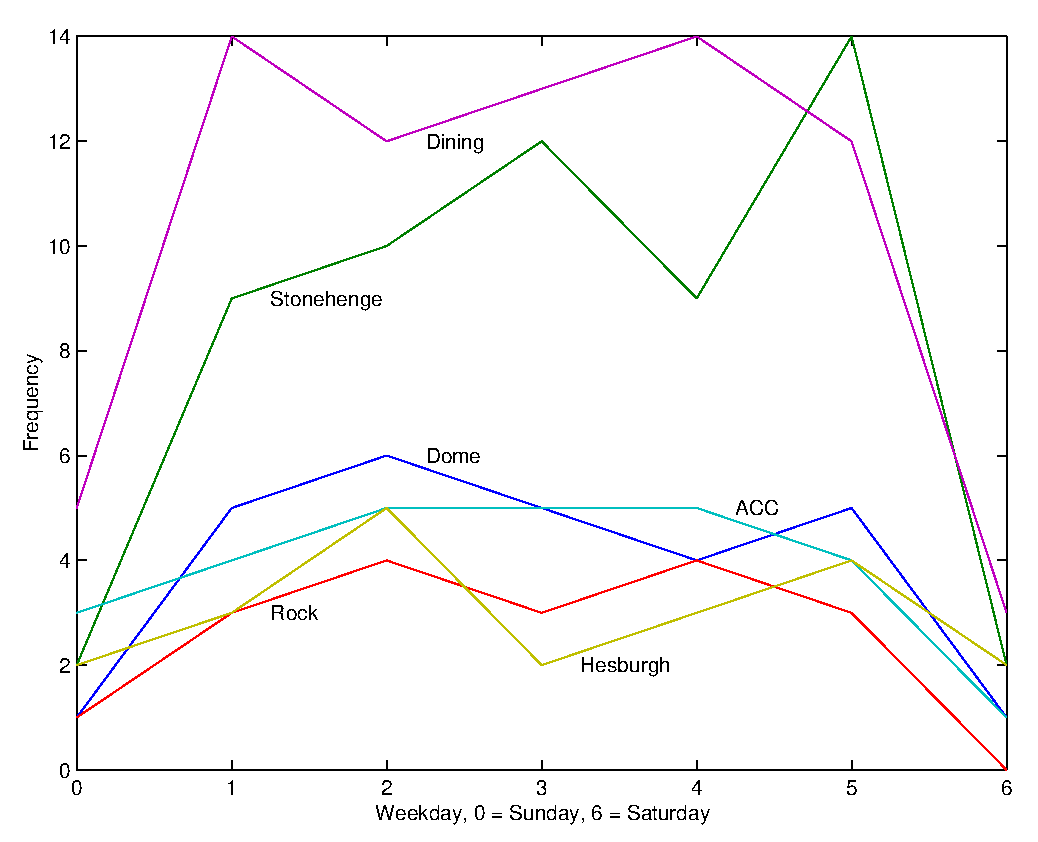
\includegraphics[scale=0.8]{sample_nd}}
%    \caption{Location distributions by day of where, where the X axis
%      is the weekday (0 through 6), and the Y axis is the sighting
%      frequency}
%    \label{fig:bogus3}
%  \end{center}
%\end{figure}
%
%Gnus typically tend to come out when there are large gatherings of
%humans with food.  Gnus work very hard at providing us with all the
%things that we like (trees, dirt, air, etc.), and so we should freely
%give them food.  They will come up and stand a respectful distance
%away from you, waiting to see if they will be rewarded for their
%efforts.  If you offer some food, they will take it and back off a
%respectful distance in order to consume their food while leaving you
%to your ``personal space.''  

%\section{Groovin' Gnus}
%\label{sec:groovin-gnus}
%
%Gnus do tend to stay away from humans in their normal day-to-day
%workings.  This is mainly because humans don't, for the most part,
%understand what they are doing.  If a Gnu is working, and a human
%approaches it, the Gnu will tend to drop whatever it is doing and run
%away.  This is probably do to the tendency for humans to have ``group
%meetings'' and ``productivity seminars.''  Most Gnus are deathly
%afraid of such overmanagement, and run at the slightest hint of it,
%for fear that it will cripple their real work.
%
%It is interesting, however, that Gnus have chosen an Institution of
%Higher Education for their BOO.\footnote{Base of Operations.}  It is
%often said that:
%\begin{quote}
%  Academic politics are the dirtiest, meanest, ugliest, and generally
%  the most low-down, in-your-face, and kick-em-while-they're-down than
%  anywhere else (even Washington D.C.)  because the stakes are so low.
%\end{quote}
%It has been hypothesized that the Gnus are subtly trying to affect a
%change for the better (i.e., eliminating the overmanagement problems)
%by working the very system that they are trying to change, from
%within.  That is, the graduates from Notre Dame can learn from the
%examples of the Gnus here, and run screaming (or chattering) at the
%slightest hint of overmanagement, and let the real work proceed
%unhindered.

% % uncomment the following lines,
% if using chapter-wise bibliography
%
% \bibliographystyle{ndnatbib}
% \bibliography{example}